% =====================================================================
%  CSLAP_Robust_Covering_SLIDES_explained.tex
%  A beginner-friendly teaching deck that vulgarizes the paper
%  "A Covering-Based Robust Counterpart for the CSLAP".
%
%  HOW TO COMPILE ON OVERLEAF
%  1. Create a new project, upload THIS .tex file.
%  2. Upload the figure PNGs into the SAME project. Either drop them
%     next to this file, or put them in a subfolder named  figures/ .
%     The \graphicspath below looks in both places, plus ../reports/figures/.
%     Needed images:
%        fig1_order_size.png        fig2_popularity_zipf.png
%        fig3_cooccurrence_lift.png fig4_demand_lorenz.png
%        fig5_affinity_dV.png       fig6_winregion_combine.png
%        fig6_winregion_reassign.png fig7_berner_decomposition.png
%  3. Set the compiler to pdfLaTeX. No exotic packages are used.
%  (If an image is missing, comment out its \includegraphics line; the
%   rest still compiles.)
% =====================================================================
\documentclass[11pt,aspectratio=169]{beamer}

\usetheme{CambridgeUS}
\usecolortheme{dolphin}
\setbeamertemplate{navigation symbols}{}
\setbeamertemplate{caption}[numbered]
\setbeamertemplate{theorems}[numbered]

\usepackage[T1]{fontenc}
\usepackage{lmodern}
\usepackage{amsmath,amssymb,mathtools}
\usepackage{booktabs}
\usepackage{graphicx}
\usepackage{xcolor}
\usepackage{tikz}
\usetikzlibrary{positioning,fit,backgrounds,arrows.meta}

\graphicspath{{./}{figures/}{../reports/figures/}}

% Small helper colors.
\definecolor{good}{RGB}{27,128,67}
\definecolor{bad}{RGB}{178,34,34}
\newcommand{\gt}[1]{\textcolor{good}{#1}}
\newcommand{\bd}[1]{\textcolor{bad}{#1}}
\newcommand{\term}[1]{\textcolor{blue!60!black}{\textbf{#1}}}

\title[CSLAP Robust Covering, explained]{A Covering-Based Robust Layout for Warehouses}
\subtitle{A guided, beginner-level walkthrough of the method, the two propositions, and why the result is negative}
\author{Teaching companion to the manuscript}
\institute{CSLAP robustness study}
\date{}

\begin{document}

\begin{frame}[plain]
  \titlepage
  \begin{center}\small A slow, plain-language tour. Every symbol is defined. No prior optimization background assumed.\end{center}
\end{frame}

\begin{frame}{How to read these slides}
  \begin{itemize}
    \item We build everything from zero. If you have never seen an optimization model, start here and keep going in order.
    \item \term{Blue bold} marks a term the first time it appears. A glossary repeats them at the end.
    \item Green means ``good for the method''. Red means ``bad for the method''.
    \item Every hard idea gets a tiny worked example with real small numbers.
    \item Propositions 1 and 2 each get their own block of slides: symbols first, then the statement, then the proof line by line, then a numerical example, then ``what it does and does not say''.
  \end{itemize}
\end{frame}

\begin{frame}{Outline}
  \tableofcontents
\end{frame}

\AtBeginSection[]{
  \begin{frame}{Where we are}
    \tableofcontents[currentsection]
  \end{frame}
}

% =====================================================================
\section{The warehouse and the problem}
% =====================================================================

\begin{frame}{The setting: a pick-and-pass warehouse}
  \begin{columns}
  \begin{column}{0.56\textwidth}
  \begin{itemize}
    \item A warehouse stores many \term{products} (also called SKUs, stock-keeping units).
    \item Products sit in \term{stations}: physical picking zones, each with a fixed number of storage \term{slots}.
    \item Customers send \term{orders}. An order is just a small set of products that must be collected together.
    \item To fill an order, a tote travels and stops at every station that holds at least one product of that order. Each stop is a \term{visit}.
  \end{itemize}
  \end{column}
  \begin{column}{0.44\textwidth}
  \centering
  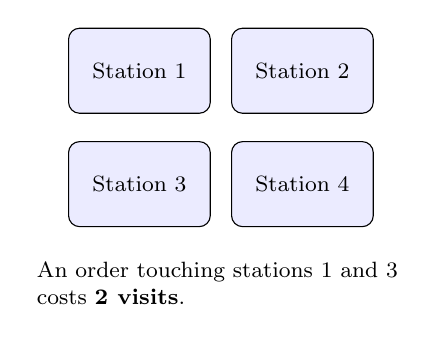
\begin{tikzpicture}[scale=0.9, every node/.style={font=\footnotesize}]
    \draw[rounded corners,fill=blue!8] (0,0) rectangle (2,1.2) node[midway]{Station 1};
    \draw[rounded corners,fill=blue!8] (2.3,0) rectangle (4.3,1.2) node[midway]{Station 2};
    \draw[rounded corners,fill=blue!8] (0,-1.6) rectangle (2,-0.4) node[midway]{Station 3};
    \draw[rounded corners,fill=blue!8] (2.3,-1.6) rectangle (4.3,-0.4) node[midway]{Station 4};
    \node[align=left] at (2.1,-2.4) {An order touching stations 1 and 3\\ costs \textbf{2 visits}.};
  \end{tikzpicture}
  \end{column}
  \end{columns}
\end{frame}

\begin{frame}{What we are allowed to decide, and what we want}
  \begin{block}{The decision}
  We choose the \term{layout}: which station each product is stored in. One product goes to exactly one station. Write the layout as a map $a$, so $a(p)$ is the station holding product $p$.
  \end{block}
  \begin{block}{The goal}
  Place correlated products together. If two products are often ordered together, storing them in the same station means an order containing both costs only one visit, not two. Over a whole day of orders, we want the \bd{smallest total number of visits}.
  \end{block}
  This is the \term{Correlated Storage Location Assignment Problem}, CSLAP. ``Correlated'' because the whole game is exploiting which products co-occur in orders.
\end{frame}

\begin{frame}{The one formula you must internalize: the visit count}
  For a layout $a$ and any set of products $u$, the visit count is
  \[
  v(a,u) \;=\; \big|\{\, a(p) : p \in u \,\}\big|.
  \]
  \begin{itemize}
    \item $a(p)$ is the station of product $p$. The set $\{a(p): p\in u\}$ collects the \emph{distinct} stations used by the products in $u$.
    \item The bars $|\cdot|$ mean ``count the elements of the set''. Distinct stations only: if three products of $u$ sit in the same station, that station is counted once.
    \item So $v(a,u)$ is exactly ``how many stops an order made of products $u$ forces''.
  \end{itemize}
  \begin{exampleblock}{Tiny example}
  Layout: $a(A){=}S_1,\ a(B){=}S_1,\ a(C){=}S_2$. Order $u=\{A,B,C\}$.
  Distinct stations used: $\{S_1, S_2\}$. So $v(a,u)=2$.
  \end{exampleblock}
\end{frame}

\begin{frame}{A property we will lean on: monotonicity}
  \begin{block}{Monotone means: adding products never lowers the visit count}
  If $u \subseteq u'$ (the set $u$ is contained in the bigger set $u'$), then
  \[
  v(a,u) \;\le\; v(a,u').
  \]
  \end{block}
  Why it is obviously true: a bigger order can only reach the same stations or more of them. You never \emph{remove} a stop by adding an item.
  \begin{exampleblock}{Check it}
  Same layout $a(A){=}S_1, a(B){=}S_1, a(C){=}S_2$.
  $v(a,\{A,B\})=1$ (only $S_1$). Add $C$: $v(a,\{A,B,C\})=2$. Went up, never down.
  \end{exampleblock}
  Keep this in your pocket. It is the entire engine of Proposition 1.
\end{frame}

% =====================================================================
\section{Optimization in one short lesson}
% =====================================================================

\begin{frame}{What is an optimization problem?}
  Three ingredients.
  \begin{enumerate}
    \item \term{Decision variables}: the things you choose. Here, where each product goes.
    \item \term{Objective function}: the number you want as small (or as large) as possible. Here, total visits.
    \item \term{Constraints}: rules a choice must obey to be allowed. Here, capacity and workload limits.
  \end{enumerate}
  \begin{itemize}
    \item A choice that obeys every constraint is \term{feasible}. The set of all feasible choices is the \term{feasible region}.
    \item The best feasible choice is the \term{optimal solution}; its objective value is the \term{optimum}.
  \end{itemize}
\end{frame}

\begin{frame}{Binary variables and the word MILP}
  \begin{itemize}
    \item We encode ``product $p$ goes to station $s$'' by a \term{binary variable} $x_{ps}\in\{0,1\}$: it is $1$ if yes, $0$ if no.
    \item ``$z_{os}=1$ if order $o$ uses station $s$'' is another binary variable, used to count visits.
    \item A model whose variables are integers (here $0/1$) and whose objective and constraints are linear is a \term{Mixed-Integer Linear Program}, MILP. ``Linear'' means no products of variables, only weighted sums.
    \item MILPs are hard in general, but powerful software can solve or approximate them.
  \end{itemize}
  \begin{block}{Two families of solvers we use}
  \term{Exact solvers} (CPLEX, Gurobi) can prove they found the true optimum. \term{Heuristics} and \term{metaheuristics} (Hexaly, genetic algorithms, simulated annealing) search cleverly and return a good solution fast, usually without a proof of optimality.
  \end{block}
\end{frame}

\begin{frame}{The CSLAP model, written out (and translated)}
  \[
  \min \; \sum_{o}\sum_{s} z_{os} \qquad\text{(total visits over all orders)}
  \]
  \vspace{-2mm}
  \begin{align*}
  &\sum_{s} x_{ps} = 1 &&\text{each product is stored in exactly one station}\\
  &\sum_{p} x_{ps} \le \zeta_s &&\text{a station holds at most }\zeta_s\text{ products (slots)}\\
  &x_{ps} \le z_{os} \;\;(p\in P_o)&&\text{if a product of order }o\text{ sits in }s,\text{ then }o\text{ visits }s\\
  &\sum_{p} x_{ps}\,\tfrac{L_p}{V_s} \le T_s &&\text{station }s\text{'s pick workload must fit its time budget}
  \end{align*}
  \footnotesize
  $P_o$ = products of order $o$. $\zeta_s$ = slot capacity. $L_p$ = how many pick-lines product $p$ generates (its demand). $V_s$ = picking speed of station $s$. $T_s$ = time capacity (workload budget) of station $s$. Remember the last line, the \term{workload constraint}: it returns as the villain at the end.
\end{frame}

\begin{frame}{Reading the objective once more, slowly}
  \[
  \sum_{o}\sum_{s} z_{os}
  \]
  \begin{itemize}
    \item For a single order $o$, the inner sum $\sum_s z_{os}$ counts the stations it visits. That is exactly $v(a,P_o)$ from before.
    \item Summing over all orders $o$ gives the total daily visits.
    \item Minimizing it pushes co-ordered products into shared stations. That is the storage version of \term{correlation clustering}: cut as few co-occurring pairs across station walls as possible.
  \end{itemize}
  So ``solve CSLAP'' literally means ``cluster products by how often they are bought together, subject to space and time limits''.
\end{frame}

% =====================================================================
\section{The big question: robustness to a changing future}
% =====================================================================

\begin{frame}{In-sample versus out-of-sample}
  \begin{itemize}
    \item We build the layout from a record of \term{past} orders. Call that the \term{training} set $O^{tr}$.
    \item We then operate the warehouse for weeks on \term{future} orders, the \term{test} set $O^{te}$, which we did not see when deciding.
    \item Performance on the training orders is \term{in-sample}. Performance on the future orders is \term{out-of-sample}. Only the second one pays the real bills.
  \end{itemize}
  \begin{block}{Analogy}
  Studying past exam papers (training) is useful only insofar as the real exam (test) resembles them. A layout perfectly tuned to last month can do badly next month if buying habits drift.
  \end{block}
\end{frame}

\begin{frame}{Demand shift, and the idea of robust optimization}
  \begin{itemize}
    \item \term{Demand shift}: the distribution of orders changes over time. New product pairings appear, popularities move.
    \item \term{Robust optimization} is a way to plan against uncertainty. Instead of optimizing for one guessed future, you pick a whole \term{uncertainty set} of plausible futures and optimize against the \emph{worst} case inside it.
    \item Intuition: buying insurance. You accept a small certain cost now to avoid a large uncertain cost later.
    \item The price you pay in the normal case for this protection is the \term{price of robustness}.
  \end{itemize}
\end{frame}

\begin{frame}{The hypothesis under test, in plain words}
  \begin{alertblock}{Hypothesis H1}
  If we deliberately \emph{enlarge} each past order into a bigger ``what-if'' order before optimizing, the resulting layout will survive future demand shift better than a layout fitted directly to the raw past orders, and the extra in-sample cost will stay small.
  \end{alertblock}
  \begin{itemize}
    \item ``Enlarge'' will be made precise in the next section through a covering construction.
    \item H1 is a \emph{conjecture}. The whole paper is a careful, honest test of whether it is true. Spoiler: for this problem it is not. The valuable part is understanding exactly why.
  \end{itemize}
\end{frame}

% =====================================================================
\section{The covering idea: set cover, patterns, closures}
% =====================================================================

\begin{frame}{Set cover and set partition}
  \begin{itemize}
    \item A \term{pattern} is just a small group of products, written $q$. Its size is capped at a number $\kappa$ (the Greek letter ``kappa''): $1 \le |q| \le \kappa$.
    \item A \term{set partition} of the products is a choice of patterns so that \emph{every product belongs to exactly one chosen pattern}. No gaps, no overlaps.
    \item We compute such a partition from the training orders, grouping products that tend to co-occur. The family of chosen patterns is $Q^*$.
  \end{itemize}
  \begin{exampleblock}{Example}
  Products $\{A,B,C,D,E,F\}$. One partition with $\kappa=2$:
  $q_1=\{A,B\},\ q_2=\{C,D\},\ q_3=\{E,F\}$. Each product appears once. Done.
  \end{exampleblock}
\end{frame}

\begin{frame}{The closure: how we ``enlarge'' an order}
  Given the patterns $Q^*$, the \term{closure} of an order $o$ replaces it by the union of every pattern that the order touches:
  \[
  \bar P_o \;=\; \bigcup_{\,q\in Q^*:\; q\cap P_o \neq \emptyset} q .
  \]
  \begin{itemize}
    \item ``$q\cap P_o\neq\emptyset$'' means pattern $q$ shares at least one product with the order. ``$\bigcup$'' glues those patterns together.
    \item Because the partition covers every product, the closure always contains the original order: $P_o \subseteq \bar P_o$.
  \end{itemize}
  \begin{exampleblock}{Example}
  Patterns $q_1=\{A,B\},q_2=\{C,D\}$. Order $o=\{A\}$ touches only $q_1$, so $\bar P_o=\{A,B\}$. The single-item order is enlarged to the pair, as if $B$ might come along.
  \end{exampleblock}
\end{frame}

\begin{frame}{The transform: optimize on the enlarged orders}
  \begin{enumerate}
    \item Take all training orders.
    \item Replace each one by its closure $\bar P_o$.
    \item Feed these enlarged ``pseudo-orders'' to the \emph{unchanged} CSLAP solver.
  \end{enumerate}
  \begin{itemize}
    \item The knob $\kappa$ controls how aggressive the enlargement is. At $\kappa=1$ every pattern is a single product, closures equal the original orders, and nothing changes (the \term{identity} case).
    \item Larger $\kappa$ means bigger patterns, bigger closures, a more conservative layout.
    \item We measure the realized enlargement by $\bar c$, the average closure size divided by the average order size. $\bar c=1$ means no growth; $\bar c=3$ means orders tripled in size on average.
  \end{itemize}
\end{frame}

\begin{frame}{Where do the patterns come from? (optional depth)}
  The partition is found by \term{column generation}, a standard technique for problems with astronomically many candidate groups.
  \begin{itemize}
    \item A \term{master problem} picks the best patterns from those seen so far. Its solution hands back \term{dual values} $\alpha_p,\beta_o$, which act as ``prices'' telling us which new pattern would help most.
    \item A \term{pricing problem} uses those prices to generate one promising new pattern. Repeat until no improving pattern exists.
    \item Two objectives for the master are used in the study: \term{min-max} (minimize the worst single order's pattern count) and \term{min-sum} (minimize total pattern hits). Min-sum scales better and is the one used on the large instances.
  \end{itemize}
  You do not need these mechanics to follow the rest. They only produce the partition $Q^*$.
\end{frame}

\begin{frame}{Two objects the propositions need}
  \begin{block}{The bottleneck $\Pi^*$ (``Pi-star'')}
  After building the partition, look at every training order and count how many patterns it touches. The largest such count is $\Pi^*$. It is the worst-case number of pattern-groups any single order spans.
  \end{block}
  \begin{block}{The uncertainty set $\widehat{\mathcal U}_\kappa$}
  This is the family of all product sets that can be covered by at most $\Pi^*$ patterns of the partition:
  \[
  \widehat{\mathcal U}_\kappa = \Big\{\, u \subseteq P :\ \exists\, R\subseteq Q^*,\ |R|\le \Pi^*,\ u \subseteq \textstyle\bigcup_{q\in R} q \,\Big\}.
  \]
  In words: the set of ``plausible future orders'' the method is willing to defend against. Every real training order lives inside it. It says nothing about whether \emph{future} orders will.
  \end{block}
\end{frame}

% =====================================================================
\section{Proposition 1, fully unpacked}
% =====================================================================

\begin{frame}{Proposition 1: the symbols first}
  Before the statement, here is every symbol it uses.
  \begin{itemize}
    \item $\bar P_o$: the closure of order $o$ (its enlarged version).
    \item $\mathcal B(o) = \{u : u \subseteq \bar P_o\}$: the \term{box} of order $o$. It is the collection of \emph{all} subsets of the closure. Think of it as ``every possible order you could form using only products inside $\bar P_o$''.
    \item $\mathcal A$: the \term{feasible layout set}. All layouts that obey the capacity and workload constraints.
    \item $v(a,u)$: the visit count from before.
    \item $\min_{a\in\mathcal A}$: ``choose the layout in $\mathcal A$ that makes what follows smallest''.
    \item $\max_{u\in\mathcal B(o)}$: ``inside the box, pick the sub-order that makes what follows largest'' (the adversary's move).
  \end{itemize}
\end{frame}

\begin{frame}{Proposition 1: the statement}
  \begin{block}{Robust-counterpart identity}
  \[
  \underbrace{\min_{a \in \mathcal A} \sum_{o} v(a, \bar P_o)}_{\text{(I) optimize on the closures}}
  \;=\;
  \underbrace{\min_{a \in \mathcal A} \sum_{o} \max_{u \in \mathcal B(o)} v(a, u)}_{\text{(II) optimize against the worst sub-order in each box}}
  \]
  \end{block}
  \begin{itemize}
    \item Left side (I): the practical thing we actually do. Just enlarge each order to its closure and minimize visits.
    \item Right side (II): a \term{robust optimization} problem. For each order, an imaginary adversary is allowed to reshape it into any subset of its closure to hurt us most; we choose the layout that is best against that worst case.
    \item The proposition says these two are the \emph{same problem}. Enlarging to closures \emph{is} a robust optimization, exactly, not by analogy.
  \end{itemize}
\end{frame}

\begin{frame}{Proposition 1: the proof, line by line}
  \begin{enumerate}
    \item Fix any single layout $a$. We compare the two objectives for this fixed $a$.
    \item Look at one order $o$. The adversary solves $\displaystyle\max_{u\subseteq \bar P_o} v(a,u)$: among all sub-orders of the closure, which gives the most visits?
    \item By \term{monotonicity}, bigger sets give more visits. The biggest set inside the box is the whole closure $\bar P_o$ itself.
    \item Therefore the adversary's best move is $u=\bar P_o$, and $\displaystyle\max_{u\subseteq \bar P_o} v(a,u) = v(a,\bar P_o)$.
    \item So term by term, the inside of (II) equals the inside of (I), for this $a$. Sum over all orders: the two objectives are equal for every $a$.
    \item If two functions are equal at every $a$, then minimizing them gives the same value and the same minimizer. Done.
  \end{enumerate}
  The whole proof is just: ``the worst subset of a set, for a monotone cost, is the set itself.''
\end{frame}

\begin{frame}{Proposition 1: a numerical example}
  Universe $\{A,B,C\}$, one pattern $q=\{A,B,C\}$. Order $o=\{A\}$, so closure $\bar P_o=\{A,B,C\}$.
  Layout $a$: $a(A)=S_1,\ a(B)=S_1,\ a(C)=S_2$.
  \begin{itemize}
    \item Left side (I): $v(a,\bar P_o)=v(a,\{A,B,C\})=|\{S_1,S_1,S_2\}|=2$.
    \item Right side (II): the adversary tries every subset of $\{A,B,C\}$:
    \[
    v(\{A\})=1,\ v(\{A,B\})=1,\ v(\{A,C\})=2,\ v(\{A,B,C\})=2,\dots
    \]
    The maximum is $2$, reached at the full closure.
  \end{itemize}
  Both sides equal $2$. The identity holds, exactly as the proof predicts.
\end{frame}

\begin{frame}{Proposition 1: what it does, and does not, say}
  \begin{block}{What it gives us (the good news)}
  A clean theoretical badge: our simple ``enlarge and solve'' procedure is provably a robust counterpart of the visit objective. We get robust optimization without modifying the solver.
  \end{block}
  \begin{alertblock}{The catch (read this twice)}
  The adversary's job was \emph{trivial}: monotonicity hands it the full closure with no real fight. So the robustness here is only ``defend against everything inside the box'', with the box fixed in advance. The proposition is about the \emph{training} objective. It says \bd{nothing} about whether \emph{future} orders will fall inside the box, which is the only thing that would make the layout actually better next month. That separate, unproven claim is H1.
  \end{alertblock}
\end{frame}

% =====================================================================
\section{Proposition 2, fully unpacked}
% =====================================================================

\begin{frame}{Proposition 2: the symbols first}
  \begin{itemize}
    \item $Q^*$: the partition (the chosen patterns).
    \item $\Pi^*$: the bottleneck, the largest number of patterns any training order touches.
    \item $\widehat{\mathcal U}_\kappa$: the uncertainty set, all product sets coverable by at most $\Pi^*$ patterns.
    \item ``A layout assigns a pattern $q$ \term{wholly to one station}'': every product of that pattern sits in the same station. The pattern is not split across walls.
    \item $\sup_{u\in\widehat{\mathcal U}_\kappa} v(a,u)$: the \emph{worst} visit count over all plausible future orders in the uncertainty set. (``$\sup$'' is the supremum, here just the maximum.)
  \end{itemize}
\end{frame}

\begin{frame}{Proposition 2: the statement}
  \begin{block}{Conditional worst-case visit bound}
  \emph{If} the layout $a$ stores every pattern $q\in Q^*$ wholly in a single station, \emph{then}
  \[
  \sup_{u\in\widehat{\mathcal U}_\kappa} v(a,u) \;\le\; \Pi^*.
  \]
  \end{block}
  \begin{itemize}
    \item In words: pack each pattern entirely into one station, and then no order from the whole uncertainty set can ever cost more than $\Pi^*$ visits.
    \item This is a \term{performance guarantee}: a hard ceiling on the worst case, valid for every future order the method claims to defend.
  \end{itemize}
\end{frame}

\begin{frame}{Proposition 2: the proof, line by line}
  \begin{enumerate}
    \item Take any order $u$ from the uncertainty set $\widehat{\mathcal U}_\kappa$.
    \item By the definition of that set, $u$ fits inside some collection $R$ of patterns with $|R|\le\Pi^*$: that is, $u \subseteq \bigcup_{q\in R} q$.
    \item Now use the assumption: each pattern $q$ lives wholly in one station, call it $a(q)$.
    \item Then every product of $u$ lies in one of the patterns of $R$, hence in one of the stations $\{a(q): q\in R\}$.
    \item So the distinct stations touched by $u$ are at most the stations of those patterns: $v(a,u) \le |R| \le \Pi^*$.
    \item This held for an arbitrary $u$ in the set, so the worst case over the whole set is at most $\Pi^*$. Done.
  \end{enumerate}
  The idea: if groups are unbroken, an order spanning few groups must span few stations.
\end{frame}

\begin{frame}{Proposition 2: a numerical example}
  Patterns $q_1=\{A,B\},\ q_2=\{C,D\},\ q_3=\{E,F\}$. Suppose $\Pi^*=2$ (no training order touched more than two patterns).
  Layout: $q_1\to S_1$ wholly, $q_2\to S_2$ wholly, $q_3\to S_3$ wholly.
  \begin{itemize}
    \item Take a plausible future order $u=\{A,D\}$. It touches $q_1$ and $q_2$, so $|R|=2\le\Pi^*$.
    \item Stations used: $A\in S_1$, $D\in S_2$, so $v(a,u)=2 \le \Pi^*=2$. Guarantee holds.
    \item Take $u=\{A,B,C\}\subseteq q_1\cup q_2$. Stations: $S_1,S_2$, so $v=2\le 2$. Still holds.
  \end{itemize}
  No order from the set can exceed two visits, because each crosses at most two unbroken groups.
\end{frame}

\begin{frame}{Proposition 2: why it is only ``conditional''}
  Two honest caveats, both taken seriously in the experiments.
  \begin{enumerate}
    \item \bd{The clean packing may not exist.} Slots are tight: the stations' total capacity equals the number of products. Forcing every pattern to stay whole may be infeasible. When patterns get split across stations, the clean ceiling $\Pi^*$ weakens to a looser bound.
    \item \bd{$\Pi^*$ depends on which orders we looked at.} If the partition was built on a subsample of orders, the certified $\Pi^*$ only bounds that subsample; the true full-data bottleneck can be larger. The paper labels these $\Pi_{\text{constrained}}$ and $\Pi_{\text{true}}$.
  \end{enumerate}
  So Proposition 2 is a guarantee \emph{if} you can pack patterns cleanly \emph{and} you trust $\Pi^*$. Useful as theory, fragile in practice.
\end{frame}

\begin{frame}{The two propositions, side by side}
  \begin{columns}
  \begin{column}{0.5\textwidth}
  \begin{block}{Proposition 1}
  Enlarging orders to closures \emph{is} a robust optimization of the training objective. Exact identity. Engine: monotonicity. It is about the past orders only.
  \end{block}
  \end{column}
  \begin{column}{0.5\textwidth}
  \begin{block}{Proposition 2}
  If patterns are stored unbroken, every defended future order costs at most $\Pi^*$ visits. A worst-case ceiling. Conditional on clean packing and on a trustworthy $\Pi^*$.
  \end{block}
  \end{column}
  \end{columns}
  \vspace{2mm}
  \begin{alertblock}{The gap both propositions leave open}
  Neither one promises that real future orders land inside the defended set often enough to make the layout cheaper next month. That promise is H1, and it must be tested with data, not proved. The rest of the deck is that test.
  \end{alertblock}
\end{frame}

% =====================================================================
\section{How we measure success}
% =====================================================================

\begin{frame}{Price of robustness, and out-of-sample gain}
  Compare the enlarged-layout $a_\kappa$ against the plain layout $a_0$ (same solver, same time).
  \begin{itemize}
    \item Nominal (training) cost $N(a)$ = visits on the past orders. Future cost $V^{te}(a)$ = visits on the held-out future orders.
  \end{itemize}
  \[
  \mathrm{PoR}(\kappa) = \frac{N(a_\kappa)-N(a_0)}{N(a_0)},
  \qquad
  G(\kappa) = \frac{V^{te}(a_0)-V^{te}(a_\kappa)}{V^{te}(a_0)}.
  \]
  \begin{itemize}
    \item \term{Price of robustness} $\mathrm{PoR}$: how much \emph{more} the enlarged layout costs on the past. Positive means we paid a price.
    \item \term{Out-of-sample gain} $G$: how much \emph{less} the enlarged layout costs on the future. \gt{Positive $G$ is the win H1 predicts.} Negative $G$ means the enlargement hurt the future too.
  \end{itemize}
\end{frame}

\begin{frame}{A fairer metric: total cost over the whole horizon}
  Surviving one shift is not enough. The enlarged layout pays its price \emph{every day} demand is stable and only maybe saves \emph{after} a shift. So net the two over the operating horizon.
  \begin{itemize}
    \item Slot the warehouse once. Operate a fraction $\tau$ of the horizon under the old regime (where the enlargement pays a per-order price $dN$), then an unforeseeable break to a new regime for the rest (where it may save $dV$ per order).
  \end{itemize}
  \[
  \mathrm{Net}(\alpha,\tau) = (1-\tau)\,dV - \tau\,dN,
  \qquad
  \text{worth it} \iff \tau < \tau^\star = \frac{dV}{dV+dN}\ \ (\text{needs } dV>0).
  \]
  \begin{itemize}
    \item $\alpha$ measures how big the future break is. $\tau^\star$ is the longest stable stretch for which buying the insurance still pays off.
    \item If $dV\le 0$ (no future saving at all), there is no $\tau$ that works. The insurance is never worth it.
  \end{itemize}
\end{frame}

% =====================================================================
\section{The datasets: what we tested on and how we built them}
% =====================================================================

\begin{frame}{A map of every dataset in the study}
  \footnotesize
  \begin{table}\centering
  \begin{tabular}{@{}llrrl@{}}
  \toprule
  Dataset & Type & SKUs & Orders & Used for\\
  \midrule
  \textbf{ISCF (baseline)} & real industrial & $4{,}328$ & $418{,}849$ & source of the derived sets; realism checks\\
  iscf480 & derived (subset) & $480$ & $\sim\!310{,}000$ & Experiment 2 (clean instance)\\
  iscf10kt & derived (subsample) & $4{,}328$ & $\sim\!10{,}000$ & temporal-split robustness checks\\
  iscfco & derived (rebuilt) & $1{,}600$ & $15{,}000$ & co-occurrence / demand-shift round\\
  syn\_50sku & synthetic (Zhang) & $50$ & varies & Experiment 1 (synthetic shift)\\
  iscf\_affinity & synthetic (planted) & $800$ & $\sim\!6{,}000$/cell & Experiment 3 (stress-test)\\
  BERNER (top-2000) & real industrial & $2{,}000$ & $\sim\!225{,}000$ & Experiment 4 (decomposition)\\
  \bottomrule
  \end{tabular}
  \end{table}
  \begin{itemize}
    \item The top four all descend from one real warehouse record, the \term{ISCF baseline}. The next two are synthetic. The last is a second real warehouse (BERNER).
    \item We introduce the baseline and its two derived testbeds now; each experiment's own dataset is introduced just before its results.
  \end{itemize}
\end{frame}

\begin{frame}{The baseline: the ISCF warehouse record (real data)}
  \begin{columns}
  \begin{column}{0.56\textwidth}
  \begin{itemize}
    \item \term{ISCF} is a real industrial slotting record. Everything else is built from it or compared against it.
    \item \textbf{Size}: $4{,}328$ unique products (SKUs), $418{,}849$ orders.
    \item \textbf{Layout}: $8$ uniform stations of $541$ slots each. The slot counts sum to exactly $4{,}328$, the number of products, so capacity does not depend on $\kappa$ (it is \term{$\kappa$-invariant}). This is why ISCF is the clean instrument.
    \item \textbf{Orders}: mean size $2.38$ products; about $55\%$ are single-item.
  \end{itemize}
  \end{column}
  \begin{column}{0.44\textwidth}
  \begin{itemize}
    \item \textbf{Demand}: very skewed. Gini $\approx 0.77$, Zipf popularity, the busiest SKU in roughly $39{,}000$ orders, a typical product in only about $38$ multi-item orders.
    \item \textbf{Co-occurrence}: sparse and mostly a popularity by-product (median pair lift $\approx 0.64$; only about a quarter of popular pairs have lift above $2$).
  \end{itemize}
  \vspace{1mm}
  \footnotesize That last point is the seed of the whole negative result: there is little genuine affinity to exploit.
  \end{column}
  \end{columns}
\end{frame}

\begin{frame}{Derived set 1: iscf10kt (a faithful small subsample)}
  \begin{block}{What it is}
  A small slice of the baseline: about $10{,}000$ orders instead of $419{,}000$, keeping \emph{all} $4{,}328$ products and the real order-ID values so that an early/late temporal split still makes sense.
  \end{block}
  \begin{block}{How it was built (\texttt{iscf\_subsample.py})}
  A plain $2.4\%$ random sample would miss about a third of the mid-popularity products, breaking coverage. So instead:
  \begin{enumerate}
    \item \textbf{Coverage skeleton}: greedily add orders until every single SKU appears at least once.
    \item \textbf{Size-stratified fill}: fill the rest so the order-size histogram and the popularity ranking match the baseline.
  \end{enumerate}
  Same $8\times541$ $\kappa$-invariant layout; workload recomputed on the smaller stream.
  \end{block}
  \textbf{Why}: to run the heavier higher-$\kappa$ temporal experiments quickly while still covering the full product universe. Temporal folds further cap the train side at $500$ to $2{,}000$ orders.
\end{frame}

\begin{frame}{Derived set 2: iscfco (a denser, co-occurrence-rich rebuild)}
  \begin{block}{Why build it}
  The baseline is $55\%$ singletons with sparse co-occurrence, so there is almost no correlation for the method to learn. To give H1 a fairer arena we rebuilt a denser instance, still grounded in the real orders.
  \end{block}
  \begin{block}{How it was built (\texttt{iscf\_cooc\_builder.py})}
  \begin{enumerate}
    \item Keep the $1{,}600$ SKUs with the highest multi-item frequency (trim the rare tail).
    \item Restrict every real order to that universe and sample $15{,}000$ orders, with the singleton share \emph{capped at $20\%$} (versus $55\%$ in the baseline).
    \item Front-load a coverage skeleton so the whole universe appears early, meaning every train/test cut from 50/50 to 90/10 has all products on the train side.
  \end{enumerate}
  \end{block}
  \textbf{Result}: $1{,}600$ SKUs, $15{,}000$ orders, $\sim\!20\%$ singletons, mean size $\sim\!3.5$, dense co-occurrence (median co-occurrence about $13$), flat $8$-station $\kappa$-invariant layout. It hosted the demand-shift round, which reached break-even and pointed us to the planted-affinity stress-test.
\end{frame}

% =====================================================================
\section{Is the data realistic? (so the test is fair)}
% =====================================================================

\begin{frame}{Why we first check the data}
  A negative result is only meaningful if the data is real warehouse data, not a toy. We checked the baseline ISCF order stream against known retail regularities. Each of the next figures supports ``this is genuine, well-behaved demand data''.
  \begin{itemize}
    \item \term{Lift} of a product pair = how much more often they co-occur than pure chance would predict. Lift $\approx 1$ means ``no special affinity beyond popularity''. Lift $\gg 1$ means ``true correlation''.
    \item \term{Gini coefficient} and \term{Lorenz curve}: standard measures of how unequal demand is across products (a few blockbusters, a long tail).
    \item \term{Zipf law}: popularity falls off in a characteristic straight line on a log-log plot, seen everywhere in retail.
  \end{itemize}
\end{frame}

\begin{frame}{Figure: order-size distribution}
  \begin{columns}
  \begin{column}{0.62\textwidth}
  \centering
  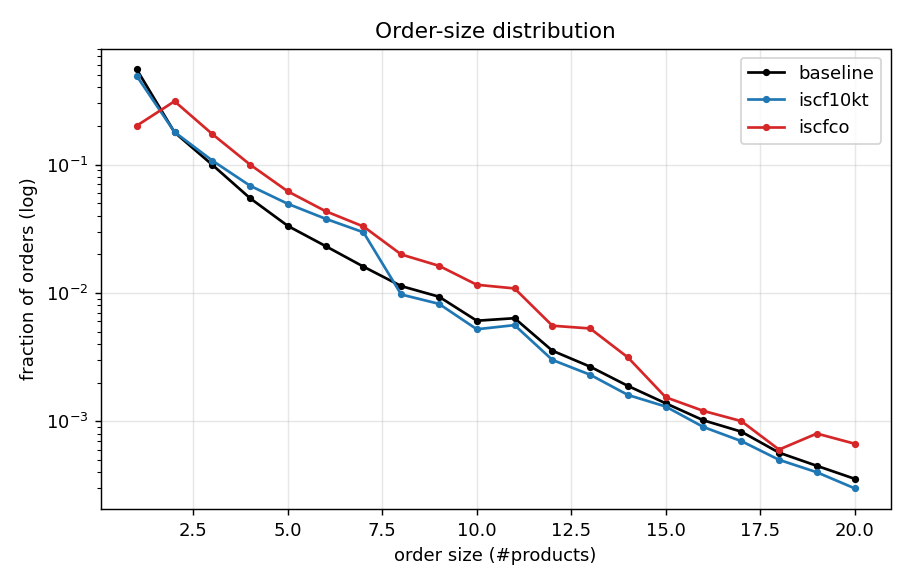
\includegraphics[width=\linewidth]{fig1_order_size.png}
  \end{column}
  \begin{column}{0.38\textwidth}
  \footnotesize
  How many products a typical order contains. Heavily skewed toward tiny orders, many singletons, a long thin tail of large baskets. This matches real picking data and matters: tiny orders give the enlargement little co-occurrence to exploit.
  \end{column}
  \end{columns}
\end{frame}

\begin{frame}{Figure: popularity follows Zipf}
  \begin{columns}
  \begin{column}{0.62\textwidth}
  \centering
  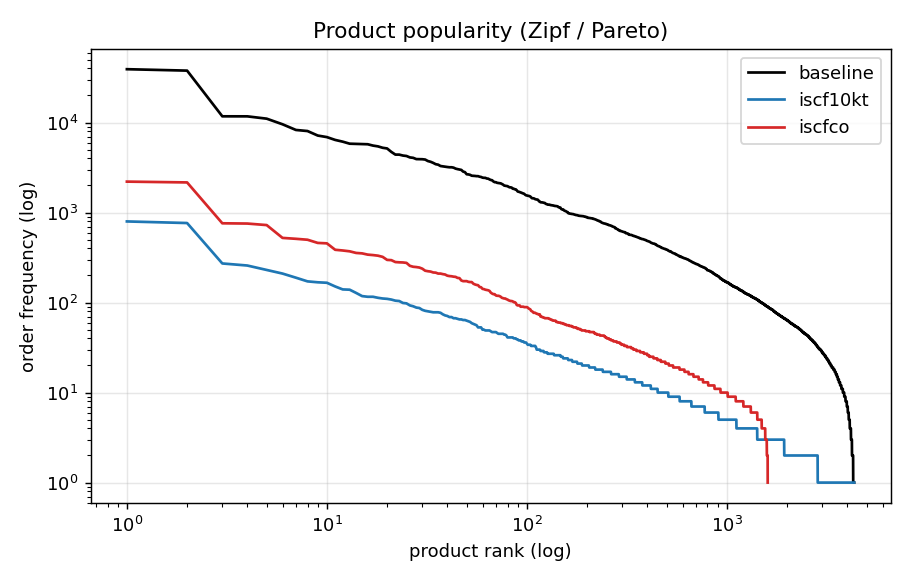
\includegraphics[width=\linewidth]{fig2_popularity_zipf.png}
  \end{column}
  \begin{column}{0.38\textwidth}
  \footnotesize
  Product popularity ranked from most to least, on a log-log scale. The near-straight line is the Zipf signature: a handful of products dominate demand, most are rare. Realistic, and it means co-occurrence is driven largely by a few popular items.
  \end{column}
  \end{columns}
\end{frame}

\begin{frame}{Figure: co-occurrence lift (the decisive diagnostic)}
  \begin{columns}
  \begin{column}{0.6\textwidth}
  \centering
  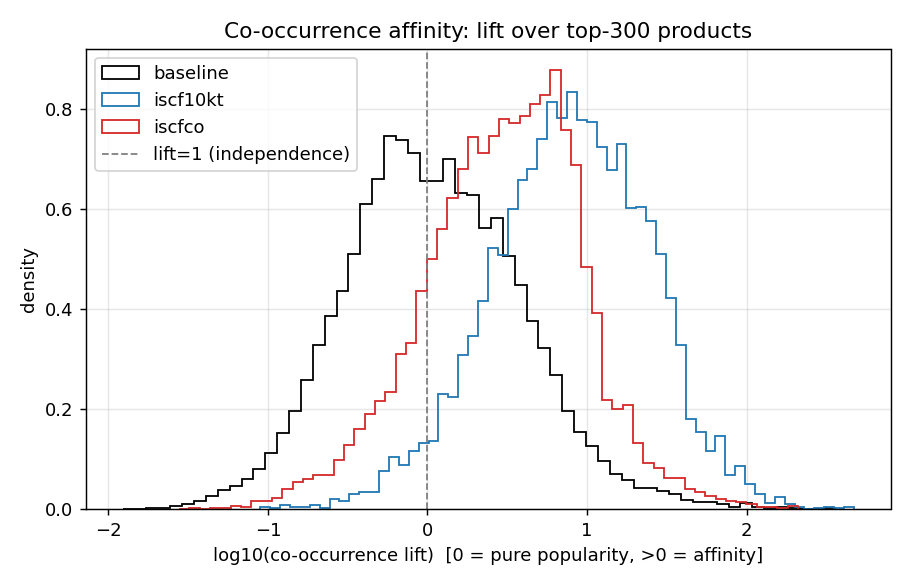
\includegraphics[width=\linewidth]{fig3_cooccurrence_lift.png}
  \end{column}
  \begin{column}{0.4\textwidth}
  \footnotesize
  Distribution of pairwise lift among popular products. It piles up near $1$. Translation: most ``co-occurrence'' is just two popular items showing up together by chance, \bd{not} a stable special affinity. There is little genuine correlation structure for the enlargement to lock onto. This is the first clue to the negative result.
  \end{column}
  \end{columns}
\end{frame}

\begin{frame}{Figure: demand inequality (Lorenz, Gini $\approx 0.77$)}
  \begin{columns}
  \begin{column}{0.6\textwidth}
  \centering
  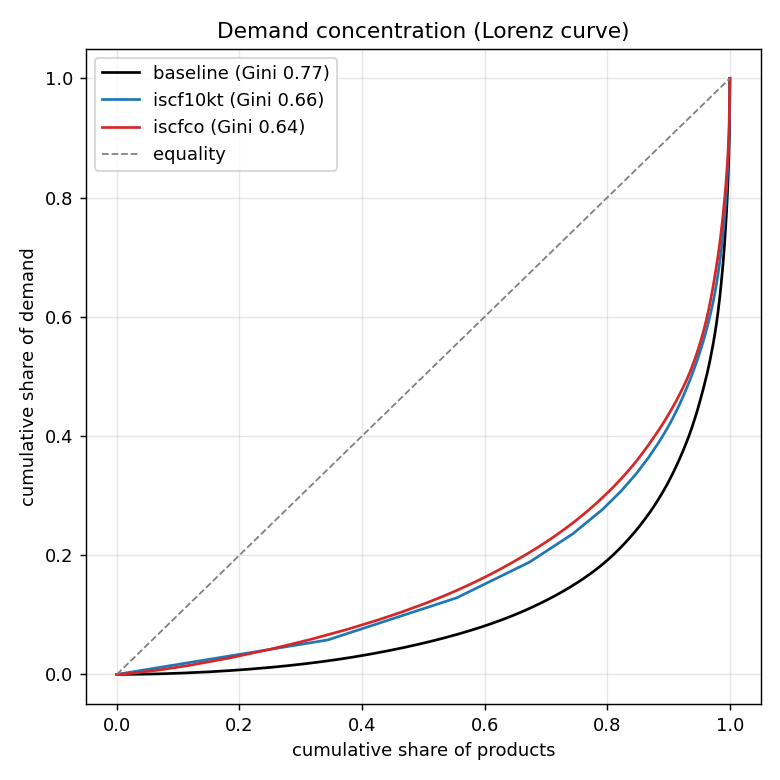
\includegraphics[width=\linewidth]{fig4_demand_lorenz.png}
  \end{column}
  \begin{column}{0.4\textwidth}
  \footnotesize
  The Lorenz curve bows far from the diagonal; the Gini coefficient is about $0.77$. A small share of products carries most of the demand. This is exactly the inequality real warehouses show, confirming the data is representative. The data is realistic; it is simply the wrong regime for the method, as the next sections show.
  \end{column}
  \end{columns}
\end{frame}

% =====================================================================
\section{Results: four honest experiments}
% =====================================================================

\begin{frame}{Dataset for Experiment 1: \texttt{syn\_50sku} and its shift}
  \begin{block}{The instance}
  A small synthetic instance of $50$ SKUs generated by the demand-correlation-pattern generator of Zhang et al. (2019), which plants common item-sets so products co-occur in a controlled way. This is the early synthetic family, later retired in favor of the real ISCF and BERNER tests.
  \end{block}
  \begin{block}{How the shift was made (against which baseline)}
  The baseline shifted is each training seed's own \texttt{syn\_50sku} order set. We freeze the product and station files and \emph{regenerate only the orders} for the future period. A shift is indexed by two knobs:
  \begin{itemize}
    \item $\theta'$, the item-set injection probability, in $\{0.5, 0.7, 0.9\}$;
    \item $\rho$, the resampling fraction, in $\{0, 0.5, 1.0\}$, where $\rho=1$ fully replaces the correlation structure over the same products.
  \end{itemize}
  Test grid: $3 \times 3 \times 5$ seeds $=45$ shifted future cells, run against $3$ training seeds $\{42,142,242\}$.
  \end{block}
\end{frame}

\begin{frame}{Experiment 1: synthetic shift, a stable price but an unstable gain}
  On \texttt{syn\_50sku} we measured PoR and $G$ across three random seeds.
  \begin{table}\centering\small
  \begin{tabular}{@{}llrl@{}}
  \toprule
  Solver & $\kappa$ & Mean $G$ (\%) & sign across 3 seeds\\
  \midrule
  Heuristic & 2 & $+0.03$ & $+\,/\,-\,/\,+$\\
  Simulated annealing & 2 & $-0.03$ & $+\,/\,-\,/\,-$\\
  \textbf{Genetic algorithm} & \textbf{2} & \gt{$+0.58$} & $+\,/\,+\,/\,+$\\
  Genetic algorithm & 3 & $-0.37$ & $+\,/\,-\,/\,-$\\
  \bottomrule
  \end{tabular}
  \end{table}
  \begin{itemize}
    \item The \emph{price} was always positive and stable (the enlargement reliably costs something on training).
    \item The \emph{gain} was tiny and mostly not repeatable. Only one cell stayed positive across seeds, and even it did not survive the cleaner tests below. No dependable out-of-sample benefit.
  \end{itemize}
\end{frame}

\begin{frame}{Dataset for Experiment 2: \texttt{iscf480}, the clean instance}
  \begin{block}{What it is and where it comes from}
  ``Company~I'' in the paper is the real ISCF baseline. For this test we use \texttt{iscf480}: the $480$ most frequent SKUs of the baseline, on the same $8$-station, slot-balanced, $\kappa$-invariant layout. It keeps the \emph{full real order stream} restricted to those products (about $310{,}000$ orders; roughly $247{,}000$ in an $80\%$ training fold).
  \end{block}
  \begin{itemize}
    \item \textbf{Why only $480$ products?} The exact CPLEX set-partition cover is provably solvable only up to a few hundred products. $480$ keeps the cover \emph{exact} while staying real data.
    \item \textbf{Why it is the clean instrument}: capacity is $\kappa$-invariant (slots fixed, workload driven by the real pick-lines), so enlarging orders cannot secretly loosen the capacity. This removes the confound that muddied the first runs.
    \item \textbf{Protocols}: repeated $5$-fold cross-validation and a $5$-cut temporal (early-train / late-test) split. Cover built per fold on training orders only; visits always counted on the real held-out orders.
  \end{itemize}
\end{frame}

\begin{frame}{Experiment 2: the clean instance, an unambiguous negative}
  On \texttt{iscf480} (Company~I) with an \emph{exact} CPLEX cover and a capacity that does not depend on $\kappa$, the two confounds of the first run are gone.
  \begin{table}\centering\small
  \begin{tabular}{@{}llrr@{}}
  \toprule
  Protocol & $\kappa$ & PoR (\%) [95\% CI] & $G$ (\%) [95\% CI]\\
  \midrule
  5-fold cross-validation & 2 & \bd{$+6.82$} $[4.79,8.84]$ & \bd{$-6.84$} $[-8.96,-4.71]$\\
  Temporal split (5 cuts) & 2 & \bd{$+5.12$} $[2.01,8.22]$ & \bd{$-7.03$} $[-10.30,-3.75]$\\
  \bottomrule
  \end{tabular}
  \end{table}
  \begin{itemize}
    \item The price is positive and the future gain is \bd{negative}, both with confidence intervals that exclude zero, every fold agreeing.
    \item Notice $\mathrm{PoR}\approx -G\approx 5\text{ to }7\%$: the enlargement costs about as much on the future as on the past. We will explain this symmetry at the end.
  \end{itemize}
\end{frame}

\begin{frame}{Interlude: the demand-shift round on \texttt{iscfco} (the exact pipeline)}
  Between the clean instance and the stress-test we gave H1 a denser arena: the co-occurrence-rich \texttt{iscfco} (introduced earlier: $1{,}600$ SKUs, $15{,}000$ orders, $20\%$ singletons, median co-occurrence $\approx 13$). The pipeline is exactly the method, end to end.
  \begin{enumerate}
    \item \textbf{Cover (CPLEX).} Per temporal fold, build the set-partition cover on the \emph{training} orders only, solved \emph{exactly} with CPLEX. Two objectives: \term{min-sum} and \term{min-max}, at $\kappa{=}1$ (identity) and $K{=}10$.
    \item \textbf{Outer-approximation.} Replace each training order by its closure $\bar P_o$, enlarging the instance.
    \item \textbf{Placement (Hexaly).} Solve CSLAP placement with Hexaly on \emph{both} the nominal ($\kappa{=}1$) and the enlarged ($K{=}10$) instances, same solver, same budget.
    \item \textbf{Evaluate on a shifted future.} Count visits on the real held-out orders after a controlled \term{demand shift}: a weight-proportional resample toward a log-normal per-product drift (order compositions stay real, $L_p$ moves; verified $L_p$ Pearson $0.997\!\to\!0.5\text{--}0.8$ as $\rho$ grows), under a flat-workload safeguard so feasibility holds. Compare PoR against $G$.
  \end{enumerate}
  \footnotesize $5$ temporal folds give $95\%$ confidence intervals. Co-occurrence-shift (structured / unstructured curveball) was run alongside; the demand mode is the one that changes $L_p$.
\end{frame}

\begin{frame}{The demand-shift round: a denser arena, the same verdict}
  On \texttt{iscfco} ($K{=}10$, demand shift swept over $\rho$). PoR is a training quantity (shift-independent); $G$ is shown at no shift and at the strongest shift.
  \begin{table}\centering\small
  \begin{tabular}{@{}lrrrr@{}}
  \toprule
  Cover & $\bar c$ & PoR (\%) [95\% CI] & $G$ at $\rho{=}0$ [CI] & $G$ at $\rho{=}2$ [CI]\\
  \midrule
  min-sum & $3.34$ & \bd{$+14.0$} $[9.9,18.2]$ & \bd{$-13.8$} $[-17.8,-9.8]$ & \bd{$-10.6$} $[-13.6,-7.5]$\\
  min-max & $\approx\!1.0^{\dagger}$ & $+2.8$ $[-5.2,10.8]$ & $-3.1$ $[-11.6,5.4]$ & $-2.8$ $[-8.0,2.4]$\\
  \bottomrule
  \end{tabular}
  \end{table}
  \footnotesize $^{\dagger}$ min-max \emph{degenerates} at $K{=}10$ on the dense instance: $4/5$ folds collapse to near-singletons (the bottleneck $\Pi\approx118$ is unbeaten in time), so it barely enlarges.
  \begin{itemize}
    \item \textbf{min-sum} builds a genuine cover ($\bar c{=}3.34$, CPLEX-certified optimal) but pays a real \bd{$+14\%$} price and \bd{loses out-of-sample}. The demand shift only nudges $G$ toward zero ($-13.8\%\!\to\!-10.6\%$), never to a significant positive; across all shift modes the best it reaches is $\approx$ break-even (unstructured $\rho{=}2$: $G=-0.6\%$, CI still excludes $0$).
    \item \textbf{min-max}'s apparent break-even is \emph{degenerate}, not protection: with $\bar c\approx1$ there is almost no enlargement to evaluate.
    \item Feasibility clean throughout (\texttt{cap\_broken}$=0$; the flat-workload safeguard held).
  \end{itemize}
  \begin{alertblock}{}
  A denser, co-occurrence-rich arena did not rescue H1. This is what pointed us to the planted-affinity stress-test (Experiment 3).
  \end{alertblock}
\end{frame}

\begin{frame}{Dataset for Experiment 3: \texttt{iscf\_affinity} (built from scratch)}
  \begin{block}{Generated, not shifted}
  Unlike Experiments 1 and 4, this data is \emph{generated from scratch} (\texttt{iscf\_affinity\_gen.py}), not a shift of a real baseline. Its marginals are calibrated to look like the real data, but its affinity is planted on purpose so the method gets its best possible chance.
  \end{block}
  \begin{columns}
  \begin{column}{0.5\textwidth}
  \footnotesize
  \textbf{Size and layout}
  \begin{itemize}
    \item $800$ SKUs split into $80$ planted \term{communities} of $10$ products that tend to be ordered together.
    \item Flat $8\times100$ stations, $\kappa$-invariant.
    \item Per cell: $\sim\!2{,}000$ training and $\sim\!4{,}000$ test orders; $3$ replicate seeds.
  \end{itemize}
  \end{column}
  \begin{column}{0.5\textwidth}
  \footnotesize
  \textbf{Realistic marginals, planted affinity}
  \begin{itemize}
    \item Demand Gini $\approx 0.73$ (real is $0.77$), Zipf popularity.
    \item Within-community lift $\approx 2.6$, far above the real $\approx 1$: strong, learnable affinity.
    \item Train orders are sparse within-community fragments (mean size $3.3$, no singletons).
  \end{itemize}
  \end{column}
  \end{columns}
  \vspace{1mm}
  \footnotesize \textbf{The break (regime B)} has size $\alpha$ and two modes: \emph{combine} (future orders grow inside the same communities, realizing the closures) and \emph{reassign} (a fraction $\alpha$ of SKUs switch communities).
\end{frame}

\begin{frame}{Experiment 3: a controlled stress-test built to favor the method}
  On \texttt{iscf\_affinity} the planted communities are strong and the future ``combine'' break grows orders \emph{within} those communities, exactly the combinations the closures encode. This is the textbook best case for H1.
  \begin{table}\centering\small
  \begin{tabular}{@{}llrr@{}}
  \toprule
  Drift mode & $\alpha$ & price $dN$/order & \textbf{saving $dV$/order} [95\% CI]\\
  \midrule
  combine & 0.5 & $+0.135$ & \bd{$-0.105$} $[-0.339,+0.129]$\\
  combine & 1.0 & $+0.152$ & \bd{$-0.111$} $[-0.356,+0.134]$\\
  reassign & 1.0 & $+0.152$ & $+0.035$ $[-0.092,+0.162]$\\
  \bottomrule
  \end{tabular}
  \end{table}
  \begin{itemize}
    \item The future saving $dV$ is \bd{never significantly positive}. In the ``combine'' regime, the one designed to help, the enlargement is actually \emph{worse} on the future.
    \item We rigged the data \emph{for} the method and it still lost. That is the opposite of an unfair test.
  \end{itemize}
\end{frame}

\begin{frame}{Experiment 3: the win-region is empty (figures)}
  \begin{columns}
  \begin{column}{0.5\textwidth}
  \centering
  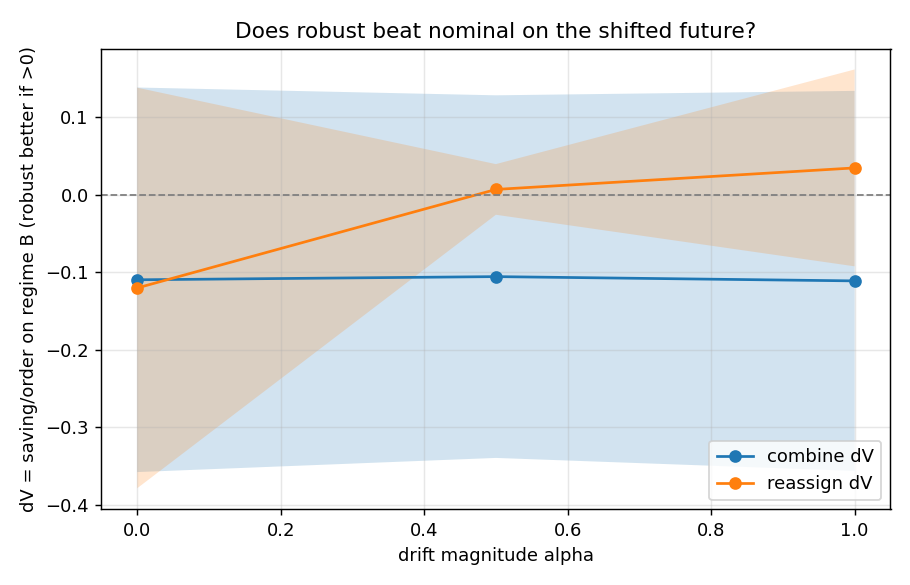
\includegraphics[width=\linewidth]{fig5_affinity_dV.png}\\
  \footnotesize The future saving $dV$ versus break size $\alpha$. It sits at or below zero with wide error bands. No regime delivers a real future gain.
  \end{column}
  \begin{column}{0.5\textwidth}
  \centering
  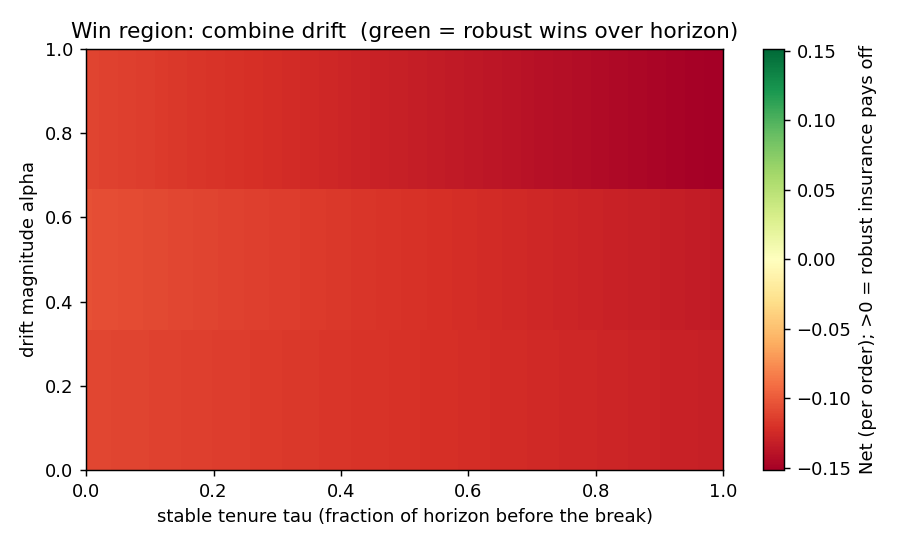
\includegraphics[width=0.92\linewidth]{fig6_winregion_combine.png}\\
  \footnotesize The total-cost map over (break size $\alpha$, stable tenure $\tau$). Green would mean ``insurance pays off''. It is essentially all red: $\mathrm{Net}<0$ almost everywhere.
  \end{column}
  \end{columns}
\end{frame}

\begin{frame}{Dataset for Experiment 4: BERNER (a second real warehouse)}
  \begin{block}{The raw data, ``Company~B''}
  BERNER is a separate real industrial order-line record: $21{,}316$ SKUs, $219{,}121$ training and $65{,}737$ test orders, $25$ physical stations with tier-based picking speeds. It is the only dataset where a positive future gain ever appeared, so it deserves the closest look.
  \end{block}
  \begin{block}{The clean rebuild we test on (\texttt{berner\_adapter.py})}
  \begin{itemize}
    \item Keep the \textbf{top $2{,}000$ SKUs} by frequency, on the real $24$-station layout (after cleaning) with the real tier speeds and the $\kappa$-invariant \emph{real} workload.
    \item \textbf{Temporal split} by order-id rank (early $10/13$ of the weeks train, late test): $175{,}419$ train and $49{,}748$ test orders.
    \item Top $2{,}000$ covers $64\%$ of train order-lines; every test product is seen in train (coverage $=1.0$).
    \item Min-sum covers built exactly with CPLEX at $\kappa\in\{2,3,4,6,10\}$, all certified optimal, enlargement $\bar c$ from $1.49$ to $3.02$.
  \end{itemize}
  \end{block}
\end{frame}

\begin{frame}{Experiment 4: the one apparent industrial win, dissected}
  On the BERNER top-$2{,}000$ instance, the earlier run showed a small positive future gain. But that run changed \emph{two} things at once: it enlarged the orders \emph{and} it quietly loosened the workload constraint $T_s$ (rebuilt from inflated closure counts). Which one caused the gain?
  \begin{block}{A clean 2-by-2 to separate them}
  Four layouts, same solver, same real test orders, only the capacity differs:
  \begin{itemize}
    \item \textbf{A} nominal orders, \emph{real} capacity (baseline).
    \item \textbf{B} closures, \emph{real} capacity. Isolates the enlargement alone.
    \item \textbf{C} closures, \emph{loose} capacity. Reproduces the old ``robust'' arm.
    \item \textbf{D} nominal orders, \emph{loose} capacity, \emph{zero enlargement}. Isolates the capacity loosening alone.
  \end{itemize}
  \end{block}
\end{frame}

\begin{frame}{Experiment 4: the decomposition table}
  \begin{table}\centering\small
  \begin{tabular}{@{}lrrrr@{}}
  \toprule
  $\kappa$ & $\bar c$ & \textbf{$G(B)$ preprocess} & $G(C)$ full & \textbf{$G(D)$ capacity-only}\\
  \midrule
  2 & 1.49 & \bd{$-3.41\%$} & $-3.11\%$ & \gt{$+0.09\%$}\\
  3 & 1.82 & \bd{$-3.65\%$} & $-0.28\%$ & \gt{$+3.37\%$}\\
  4 & 2.07 & \bd{$-2.15\%$} & $+2.05\%$ & \gt{$+4.79\%$}\\
  6 & 2.43 & \bd{$-0.93\%$} & $+3.17\%$ & \gt{$+5.41\%$}\\
  10 & 3.02 & $+0.13\%$ & $+4.56\%$ & \gt{$+7.97\%$}\\
  \bottomrule
  \end{tabular}
  \end{table}
  \begin{itemize}
    \item \textbf{B} (enlargement alone): negative to break-even. The preprocess on its own does not help.
    \item \textbf{D} (capacity alone, no enlargement): delivers the entire gain, and more than the full arm.
    \item \textbf{C} sits below \textbf{D} everywhere: adding closures \emph{drags} the result down by about $3\%$.
  \end{itemize}
\end{frame}

\begin{frame}{Experiment 4: the picture and the verdict}
  \begin{columns}
  \begin{column}{0.58\textwidth}
  \centering
  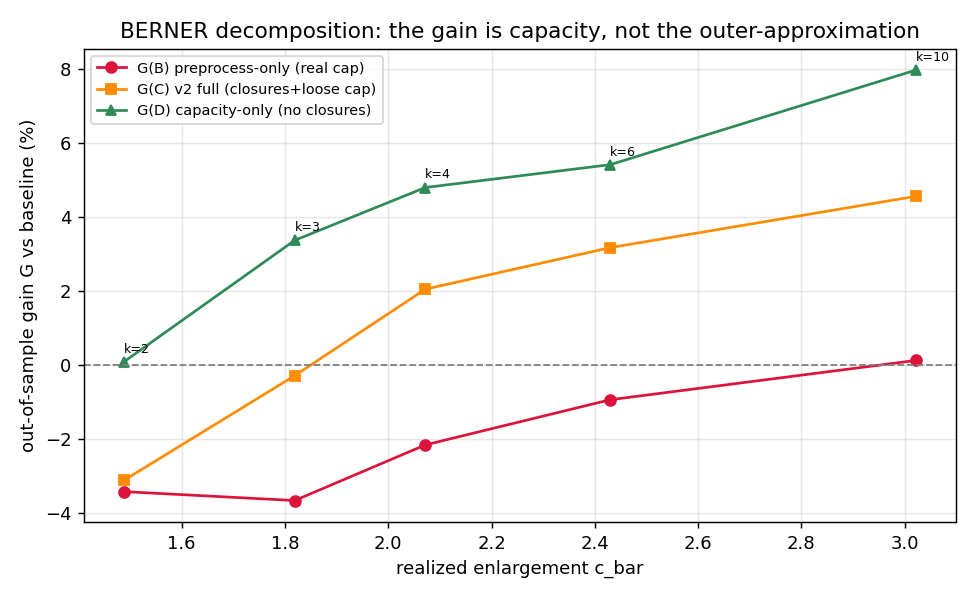
\includegraphics[width=\linewidth]{fig7_berner_decomposition.png}
  \end{column}
  \begin{column}{0.42\textwidth}
  \footnotesize
  Green (capacity-only) rises steadily. Red (preprocess-only) stays negative until a huge enlargement barely reaches zero. Orange (full) lies below green throughout.\\[2mm]
  \textbf{Verdict.} The industrial ``win'' we once celebrated came from \bd{loosening the workload limit}, a constraint relaxation that helps the plain layout just as much, \bd{not} from our outer-approximation. Once capacity is held at its real value, the enlargement returns the same negative as everywhere else.
  \end{column}
  \end{columns}
\end{frame}

% =====================================================================
\section{Why it cannot help here: the operational-research explanation}
% =====================================================================

\begin{frame}{The pattern across all four experiments}
  Synthetic shift, clean instance, rigged-favorable affinity, and the industrial decomposition all point the same way: the enlargement reaches break-even at best, and the lone positive was a different effect entirely. One mechanism explains it all. It is specific to \emph{this} objective.
\end{frame}

\begin{frame}{Step 1: the objective is already well estimated}
  \begin{itemize}
    \item Minimizing visits is correlation clustering. The optimal layout depends on the data only through aggregate \term{co-occurrence counts}: how often each product pair is bought together.
    \item Those counts are a \emph{stable, low-variance statistic}. They are averaged over hundreds of thousands of orders, so the random error in any single count is tiny compared to the differences between layouts.
    \item The plain layout therefore already sits at a solid optimum of a sharply estimated function. There is little estimation noise to clean up.
  \end{itemize}
\end{frame}

\begin{frame}{Step 2: the enlargement only adds bias}
  \begin{itemize}
    \item By Proposition 1 the enlargement is a robust counterpart, but its adversary is trivial (monotonicity). It adds no real hedging beyond making each order bigger.
    \item A bigger order is a \term{coarser, upper-bound} version of the true cost. Optimizing an upper bound pulls the layout away from the true optimum. The bigger the closures, the larger this pull. This is \term{bias}: a systematic error introduced on purpose.
  \end{itemize}
  \begin{block}{Bias and variance, the core trade}
  Any robust method trades a little \term{bias} (being deliberately off-target) for a reduction in \term{variance} (being less sensitive to noisy data). The trade is worth it only when there is enough variance to remove.
  \end{block}
\end{frame}

\begin{frame}{Step 3: bias without variance reduction is a losing trade}
  \begin{itemize}
    \item Here the variance is already small (Step 1), so there is almost nothing for the enlargement to remove.
    \item But the bias it adds is real and grows with $\kappa$ (Step 2).
    \item So the method pays bias and buys no compensating variance reduction. For this objective that trade can only move the cost the wrong way.
  \end{itemize}
  \begin{alertblock}{The signature we already saw}
  This is exactly why $\mathrm{PoR}\approx -G$ on the clean instance: the same pure bias term shows up as a cost on the training orders (the price) and as an equal cost on the future orders (the negative gain), with no variance benefit in between to offset it.
  \end{alertblock}
\end{frame}

\begin{frame}{Step 4: the careful, bounded conclusion}
  \begin{block}{What we claim}
  For an objective of this kind, a deterministic correlation-clustering placement learned from a stable, well-sampled co-occurrence statistic, enlargement-based robustification is \emph{redundant} with the direct optimizer. The plain min-visits solver already performs the very clustering the cover re-encodes, so the closures add conservatism without adding information.
  \end{block}
  \begin{itemize}
    \item We do \emph{not} claim the construction is useless for every uncertainty problem. The claim is scoped to this objective and this kind of stable data.
    \item It also explains why the ``combine'' best case was empirically the worst: growing future orders is exactly when a layout spread over more stations is punished most, and spreading is what the enlargement does.
  \end{itemize}
\end{frame}

\begin{frame}{Step 5: the industrial subtlety in one line}
  We thought we gained on the real industrial data. A more careful test, holding the workload limit fixed at its true value, proved the gain came from a \bd{loosened workload constraint}, not from the outer-approximation. A binding workload limit forces co-located products apart and inflates visits; relaxing it lets the optimizer cluster freely and lowers visits on past and future alike. That relaxation is available to the plain layout too, so it was never a property of our method.
\end{frame}

% =====================================================================
\section{Conclusion and glossary}
% =====================================================================

\begin{frame}{What to remember}
  \begin{enumerate}
    \item The construction is mathematically sound: Proposition 1 makes ``enlarge then solve'' an exact robust optimization, Proposition 2 gives a worst-case ceiling under a clean packing.
    \item Soundness of the \emph{training} problem is not the same as a benefit on the \emph{future}. That extra promise, H1, is what fails.
    \item Tested four ways, including on data built to favor it and on two real industrial instances, the enlargement gives no dependable out-of-sample gain.
    \item The one apparent industrial win was a capacity-relaxation side effect, proven by a clean 2-by-2, not the method.
    \item The reason is bias without variance reduction: the plain optimizer already captures the stable correlation structure, so enlargement only perturbs it.
  \end{enumerate}
  A clean, honest, fully explained negative result is itself a contribution.
\end{frame}

\begin{frame}{Glossary (1 of 2)}
  \footnotesize
  \begin{description}
    \item[Product / SKU] An item stored and picked.
    \item[Order] A set of products a customer wants together.
    \item[Station] A picking zone with limited slots; an order ``visits'' it if it holds one of the order's products.
    \item[Layout $a$] The decision: which station each product goes to, $a(p)$.
    \item[Visit count $v(a,u)$] Number of distinct stations the products of $u$ occupy.
    \item[Monotonicity] Adding products never lowers the visit count.
    \item[Objective / constraint / feasible] The number minimized / a rule a choice must obey / a choice obeying all rules.
    \item[MILP] Mixed-integer linear program; linear model with $0/1$ variables.
    \item[Exact solver vs heuristic] Proves optimality (CPLEX, Gurobi) vs finds a good solution fast (Hexaly, genetic algorithm, simulated annealing).
  \end{description}
\end{frame}

\begin{frame}{Glossary (2 of 2)}
  \footnotesize
  \begin{description}
    \item[Training / test] Past orders used to build the layout / future orders used to judge it.
    \item[Robust optimization] Optimize against the worst case inside an uncertainty set of plausible futures.
    \item[Pattern $q$, size cap $\kappa$] A small product group of size at most $\kappa$.
    \item[Partition $Q^*$] Patterns covering every product exactly once.
    \item[Closure $\bar P_o$] The order enlarged to the union of the patterns it touches.
    \item[Bottleneck $\Pi^*$] Largest number of patterns any training order touches.
    \item[Uncertainty set $\widehat{\mathcal U}_\kappa$] Product sets coverable by at most $\Pi^*$ patterns.
    \item[PoR / $G$] Price of robustness (extra training cost) / out-of-sample gain (future saving).
    \item[Realized enlargement $\bar c$] Average closure size over average order size.
    \item[Bias / variance] Deliberate off-target error / sensitivity to data noise; robustness trades the first for the second.
  \end{description}
\end{frame}

\begin{frame}[plain]
  \centering
  \vfill
  {\Large Thank you.}\\[2mm]
  {\normalsize Questions to ask yourself: where did monotonicity do all the work in Proposition 1? Why does a tight workload limit, once relaxed, look like robustness but is not?}
  \vfill
\end{frame}

\end{document}
